% THIS IS SIGPROC-SP.TEX - VERSION 3.1
% WORKS WITH V3.2SP OF ACM_PROC_ARTICLE-SP.CLS
% APRIL 2009
%
% It is an example file showing how to use the 'acm_proc_article-sp.cls' V3.2SP
% LaTeX2e document class file for Conference Proceedings submissions.
% ----------------------------------------------------------------------------------------------------------------
% This .tex file (and associated .cls V3.2SP) *DOES NOT* produce:
%       1) The Permission Statement
%       2) The Conference (location) Info information
%       3) The Copyright Line with ACM data
%       4) Page numbering
% ---------------------------------------------------------------------------------------------------------------
% It is an example which *does* use the .bib file (from which the .bbl file
% is produced).
% REMEMBER HOWEVER: After having produced the .bbl file,
% and prior to final submission,
% you need to 'insert'  your .bbl file into your source .tex file so as to provide
% ONE 'self-contained' source file.
%
% Questions regarding SIGS should be sent to
% Adrienne Griscti ---> griscti@acm.org
%
% Questions/suggestions regarding the guidelines, .tex and .cls files, etc. to
% Gerald Murray ---> murray@hq.acm.org
%
% For tracking purposes - this is V3.1SP - APRIL 2009

\documentclass{acm_proc_article-sp}

\usepackage[utf8]{inputenc}
\usepackage{graphicx}
\usepackage{caption}
\usepackage[]{mcode}

\begin{document}

\title{Rapport Matlab : Simulation d'une chaîne de transmission numérique sur canal gaussien à bande limitée}

\numberofauthors{2} 
\author{
\alignauthor
Hoël Boëdec\\
       \affaddr{ENSIMAG - ISSC}\\
       \affaddr{3 rue Amiral Courbet}\\
       \affaddr{Grenoble, France}\\
       \email{hoel.boedec@phelma.grenoble-inp.fr}
% 2nd. author
\alignauthor
Fournier Mickaël\\
       \affaddr{ENSIMAG - ISSC}\\
       \affaddr{22 rue Francis Jaquard}\\
       \affaddr{Grenoble, France}\\
       \email{mickael.fournier@phelma.grenoble-inp.fr}
}

\maketitle
\begin{abstract}
    
\end{abstract}

\keywords{covert channel, steganography, data hidding} % NOT required for Proceedings

\section{Introduction}

\begin{center}
\includegraphics[height=3cm]{DirtyConstellation.eps}
\end{center}


\section{Génération aléatoire des éléments binaires}
\begin{lstlisting}
N = 2048;

bn = zeros(1, N);
for k=1:1:length(bn)
    bn(k) = round(rand());
end

mean(bn);
var(bn);
\end{lstlisting}

La moyenne et la variance empirique de bn valent respectivement 0,5 et 0,25. Ceci est cohérent avec la théorie car 0 et 1 sont équiprobables.


\section{Conversion des éléments binaires en symboles (mapping)}
\begin{lstlisting}
an = zeros(1, N);
for k=1:1:length(bn)
    an(k) = 2*bn(k)-1;
end

mean(an); # 0.0
var(an); # 1

mean(an.^2); #1
\end{lstlisting}

La moyenne et la variance empirique de an valent respectivement 0 et 1. Ceci est cohérent avec la théorie car les symboles sont centrés et ???.
La puissance moyenne temporelle empirique du vecteur an vaut 1 (unité ??).

\begin{lstlisting}
D = 10000000; # 1 Mbit/sec
T = 1/D;

t_a = 0 : T : N*T - T;

plot(t_a, an, '*')
\end{lstlisting}

\begin{center}
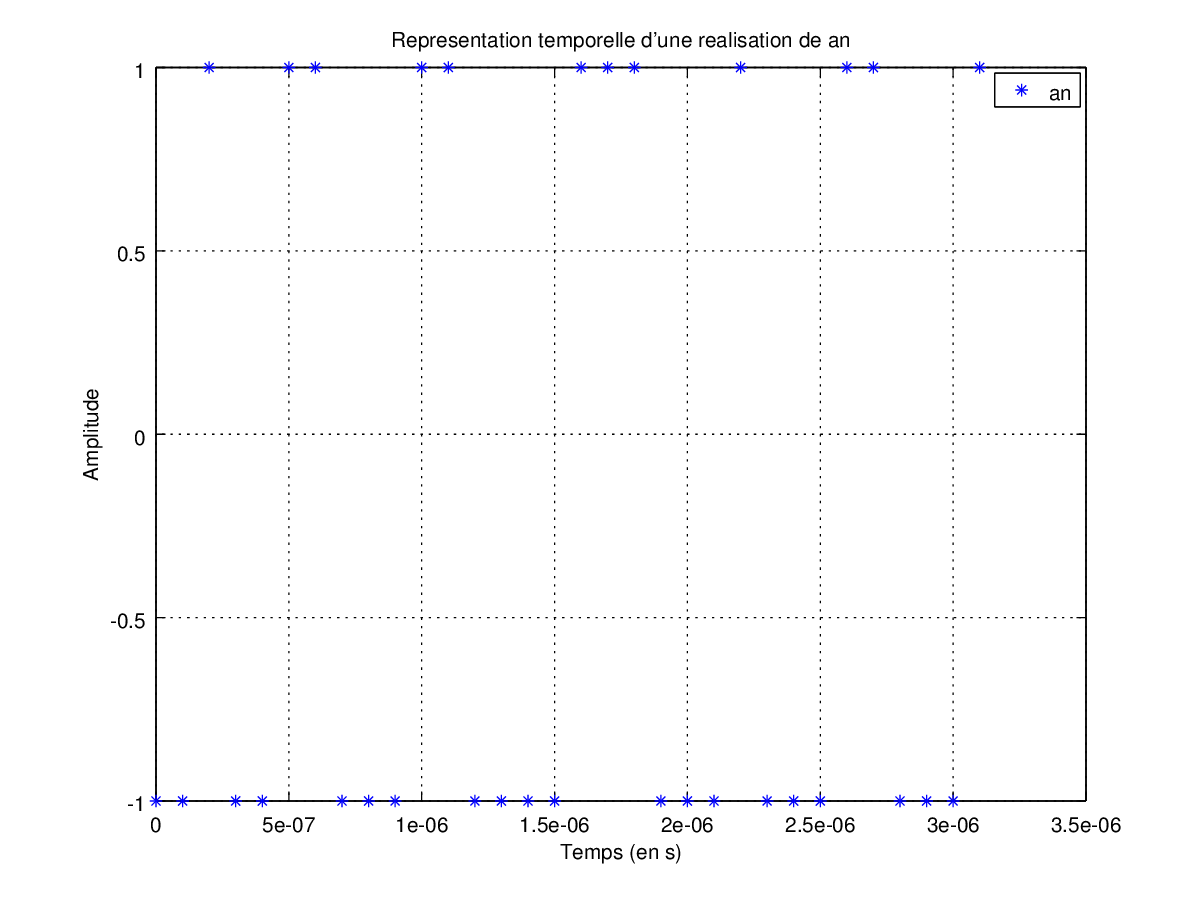
\includegraphics[scale=0.45]{ak_2.png}
\end{center}

\begin{lstlisting}
plot(real(an), imag(an), '*')
\end{lstlisting}

\begin{center}
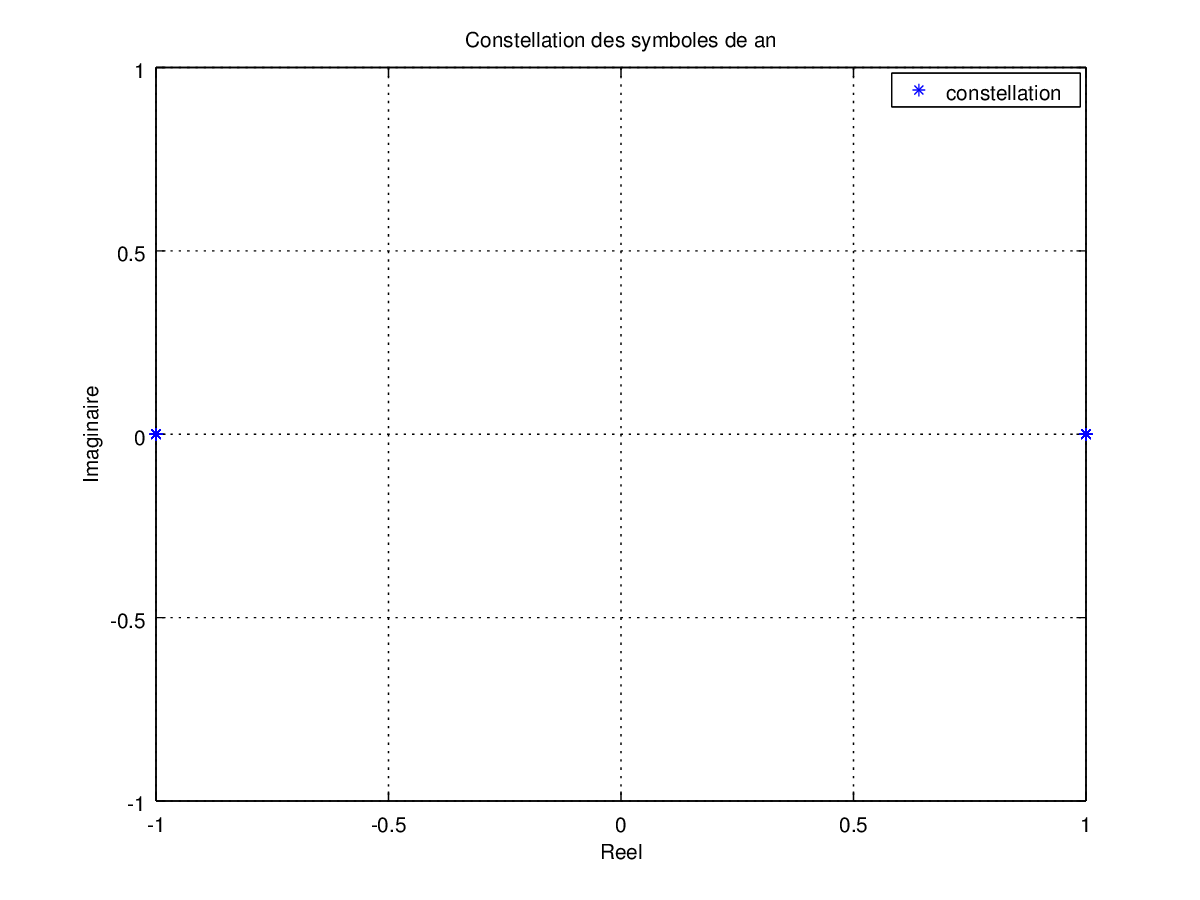
\includegraphics[scale=0.45]{constell_2.png}
\end{center}


\section{Conversion numérique - analogique}
\subsection{Expansion - Question 1}

\begin{lstlisting}
F = 16; # Facteur de surechantillonage
st = zeros(1, N*F);
st(1) = F*an(1);
for k=1:1:length(an)-1
    st(k*F+1) = F*an(k+1);
end
\end{lstlisting}

Question 1 : la durée du signal st vaut NF/D.

\begin{center}
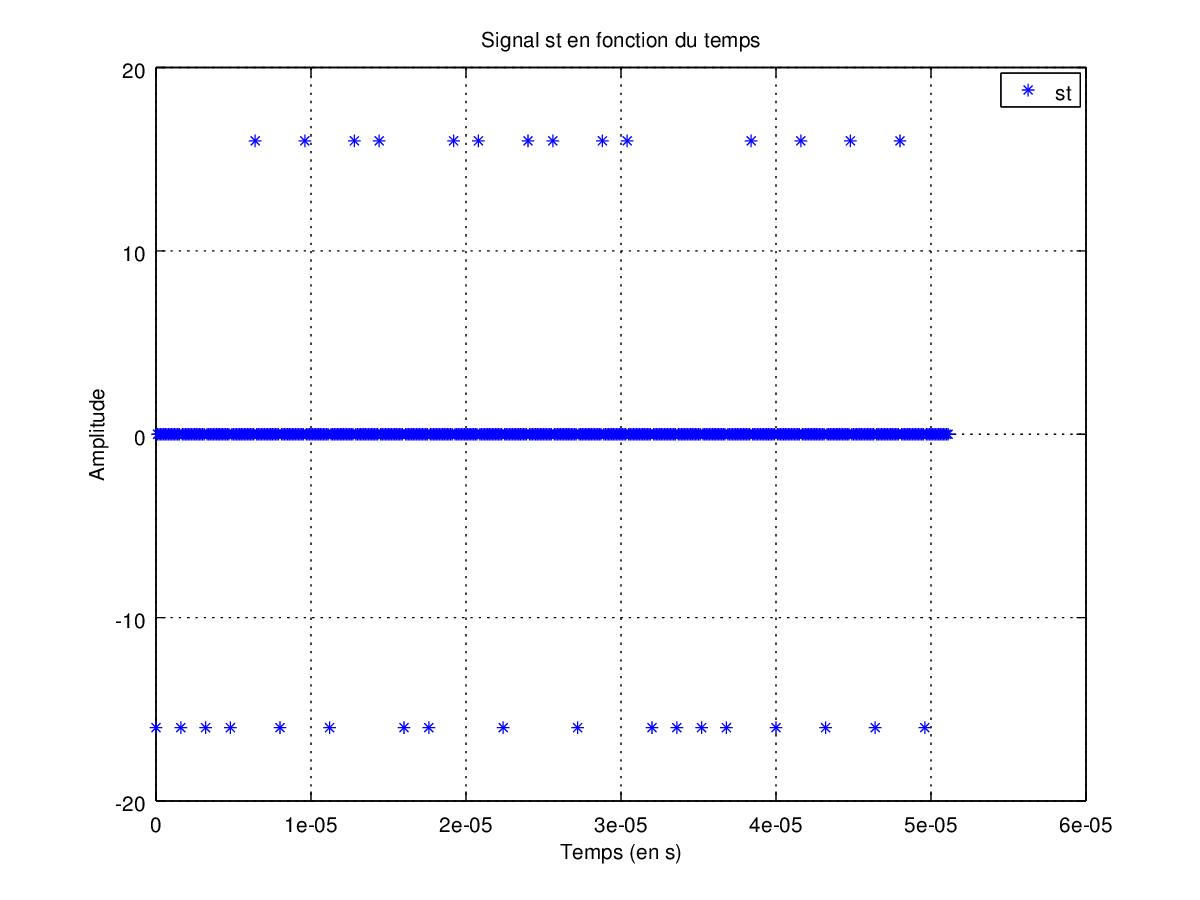
\includegraphics[scale=0.45]{st_3.png}
\end{center}

\subsection{Etude des filtres - Question 2}

\begin{lstlisting}
L = 8;
alpha = 0.5;
Te = T/F;
t_filtre = [0 : T/F : L*T -T/F];
\end{lstlisting}

\subsubsection{NRZ}

\begin{lstlisting}
s_t = gen_filters2('nrz',t_filtre,T,F,L,alpha);
plot(t_filtre, s_t, '*')
\end{lstlisting}

\begin{center}
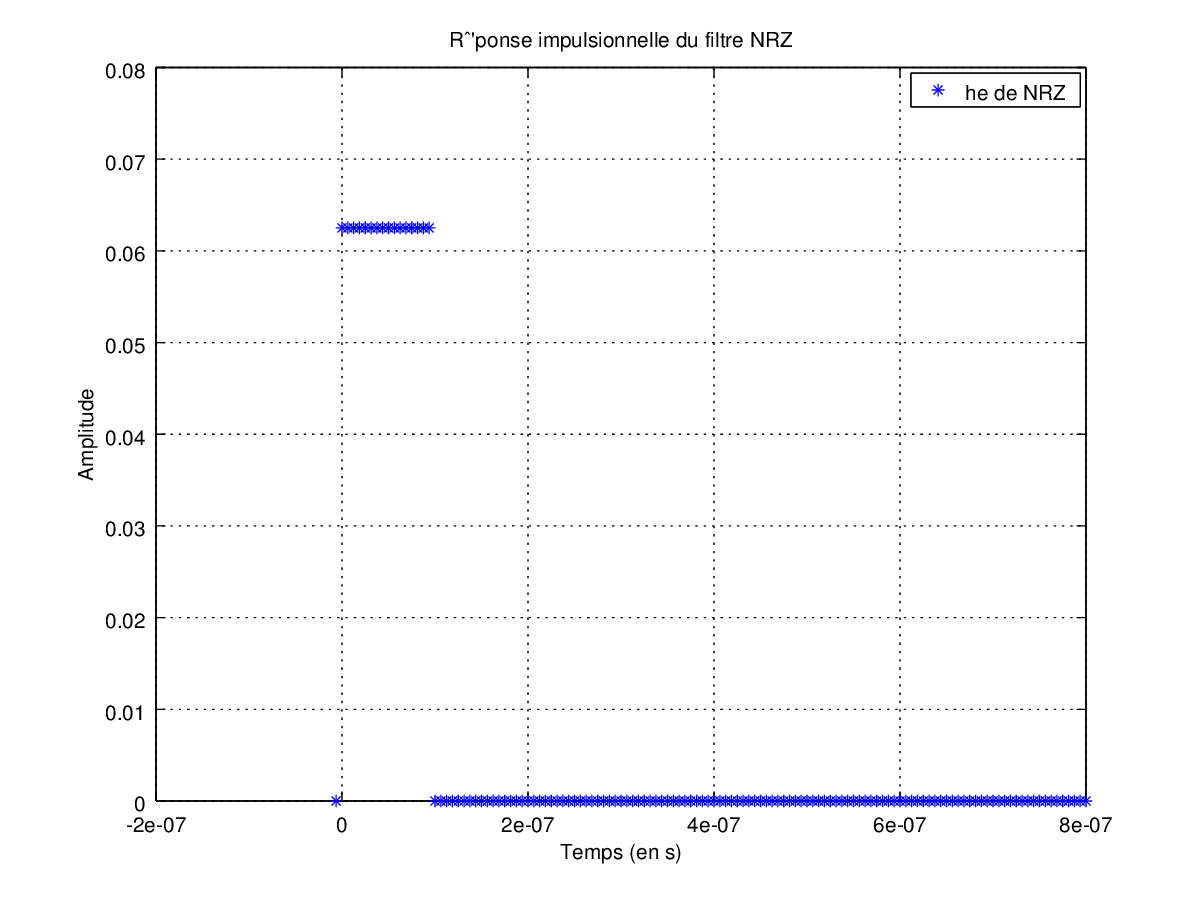
\includegraphics[scale=0.45]{NRZ_3.png}
\end{center}

\begin{center}
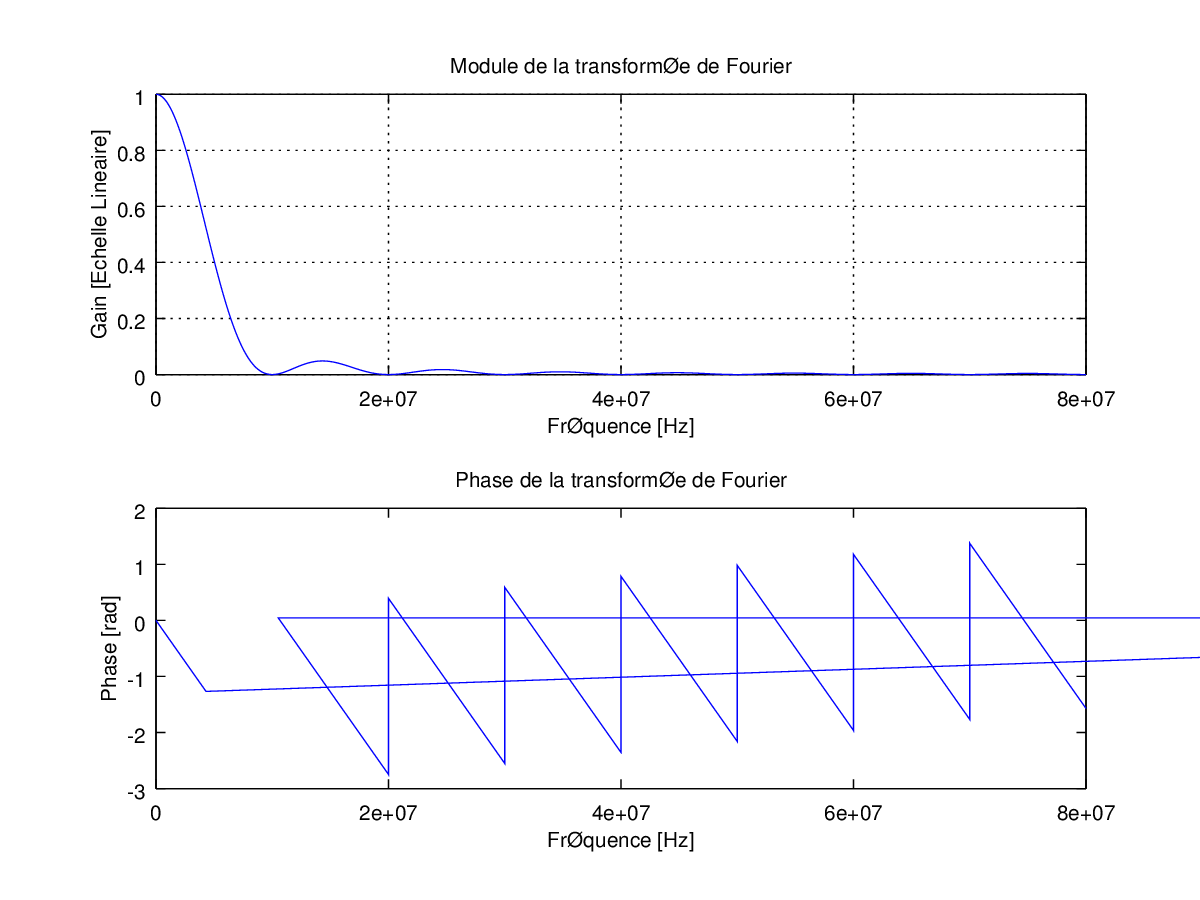
\includegraphics[scale=0.45]{NRZ_rep_3.png}
\end{center}

\subsubsection{RZ}

\begin{lstlisting}
s_t = gen_filters2('rz',t_filtre,T,F,L,alpha);
plot(t_filtre, s_t, '*')
\end{lstlisting}

\begin{center}
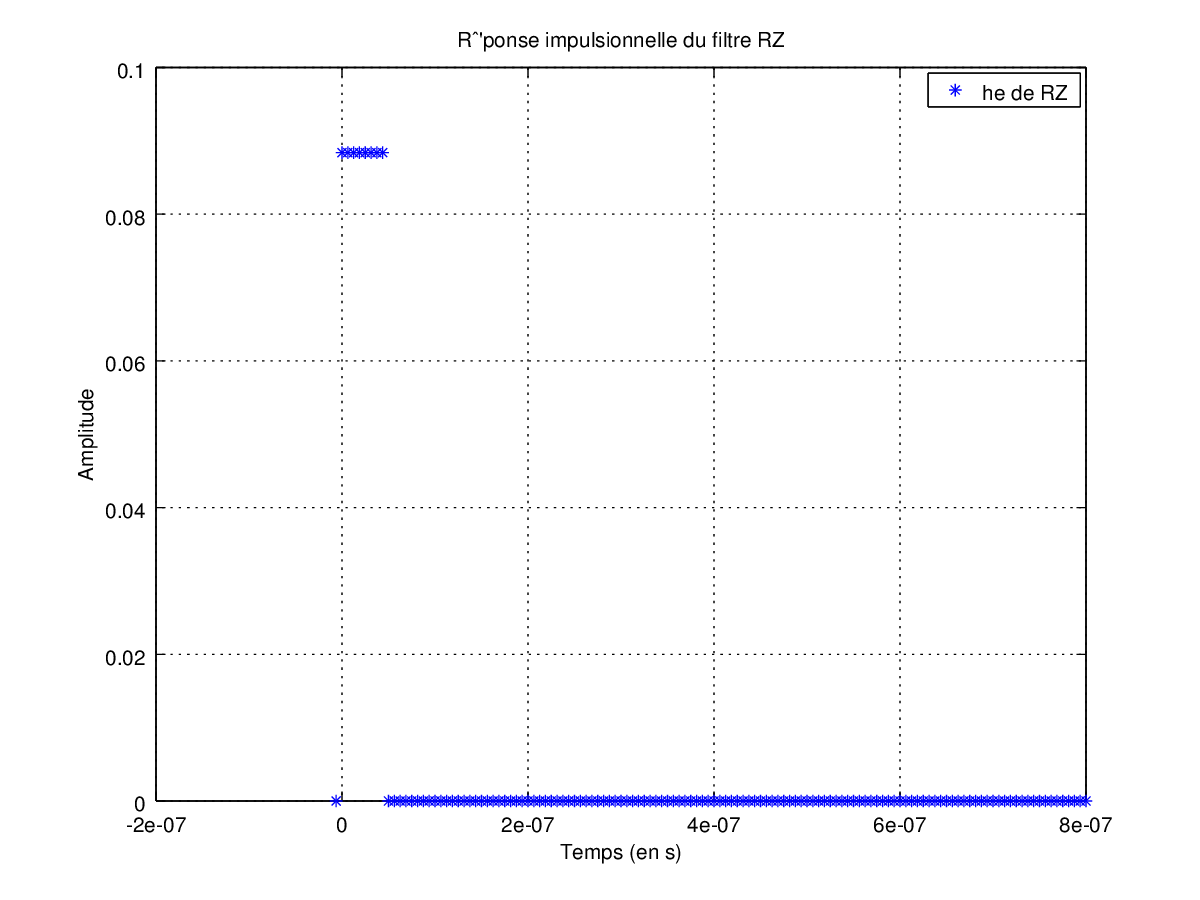
\includegraphics[scale=0.45]{RZ_3.png}
\end{center}

\begin{center}
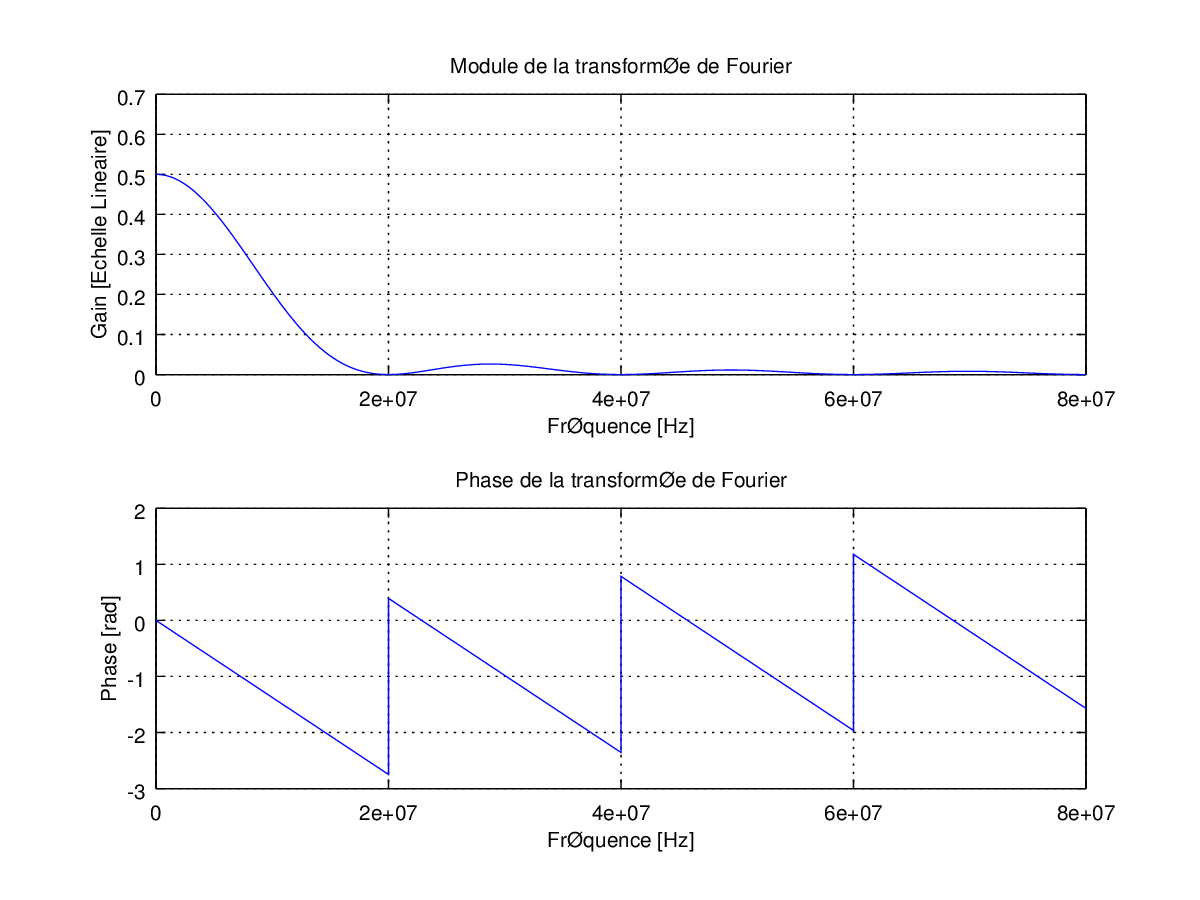
\includegraphics[scale=0.45]{RZ_rep_3.png}
\end{center}

\subsubsection{SRRC}

\begin{lstlisting}
s_t = gen_filters2('srrc',t_filtre,T,F,L,alpha);
plot(t_filtre, s_t, '*')
\end{lstlisting}

\begin{center}
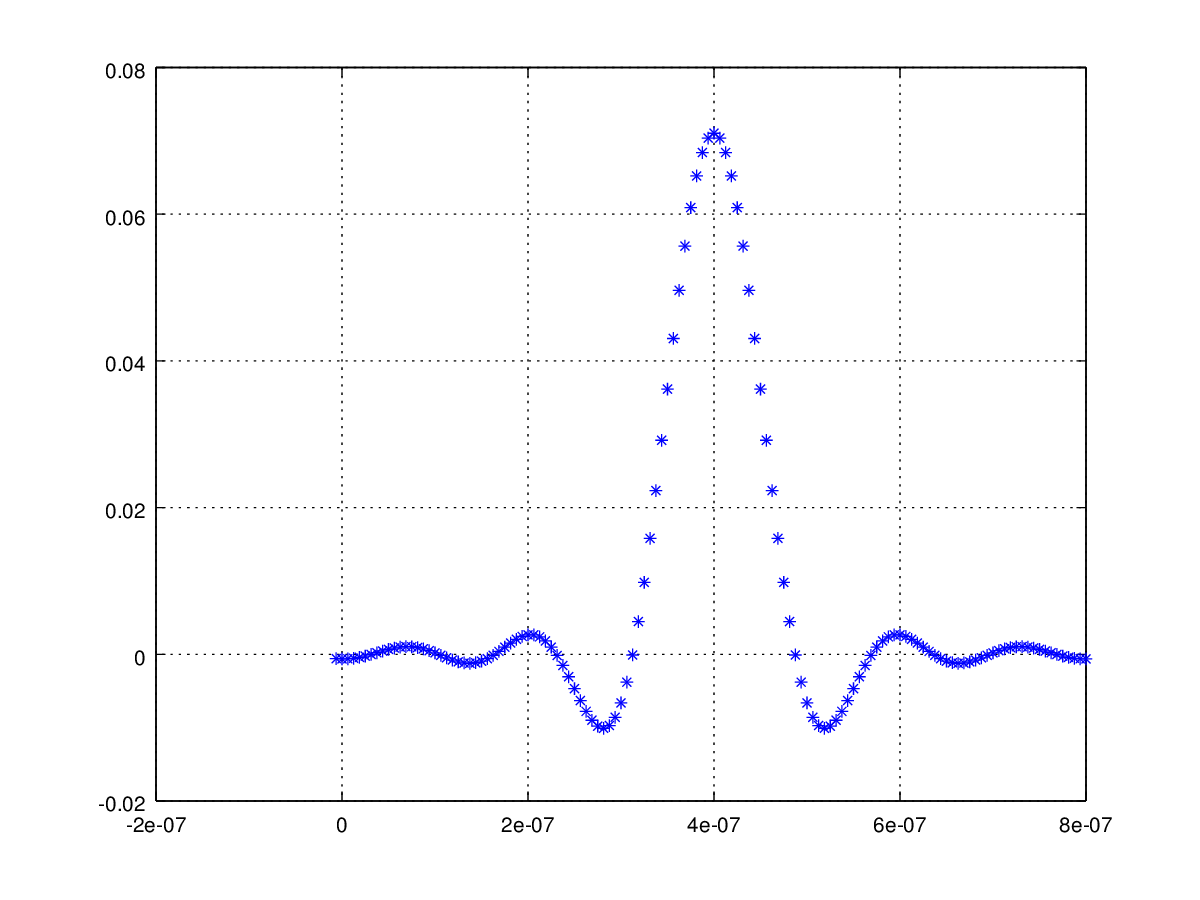
\includegraphics[scale=0.45]{SRRC_3.png}
\end{center}

\begin{center}
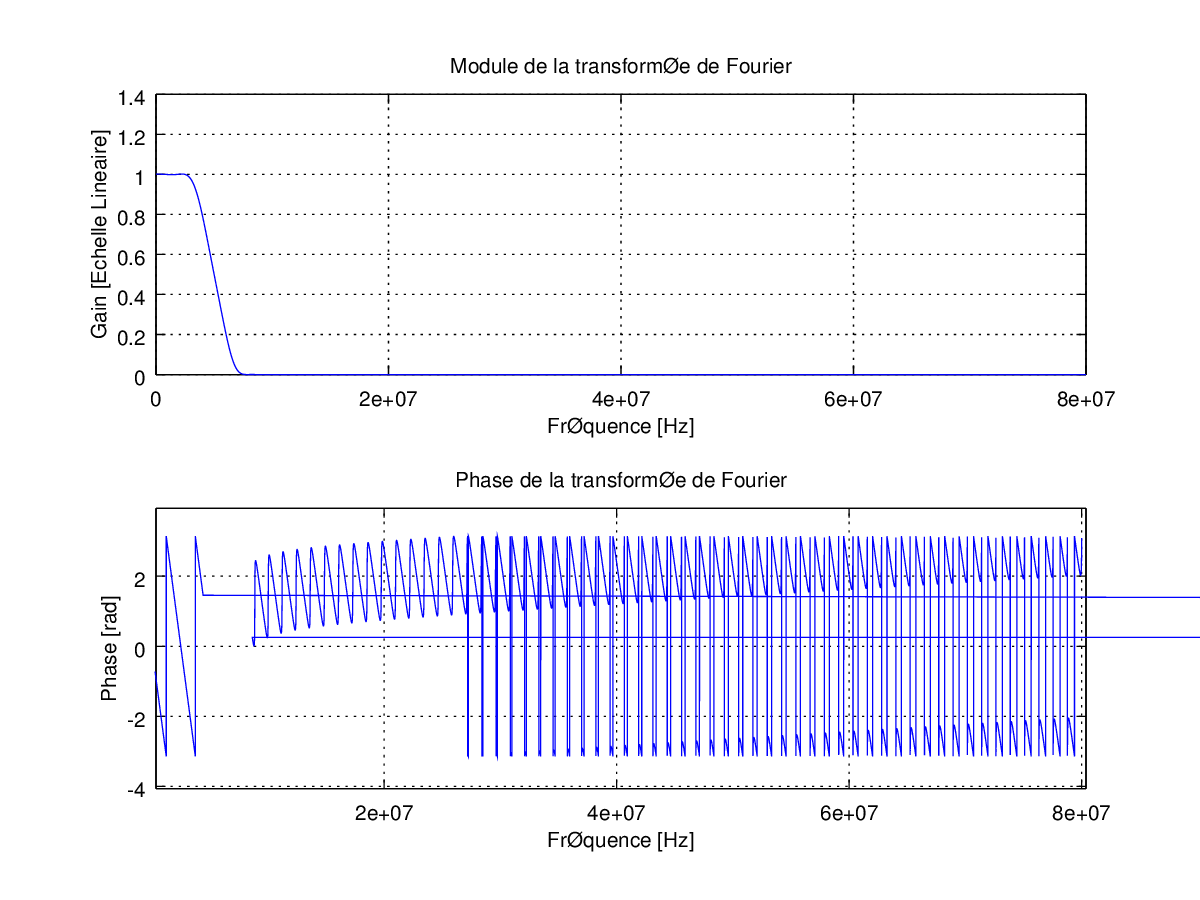
\includegraphics[scale=0.45]{SRRC_rep_3.png}
\end{center}

\begin{center}
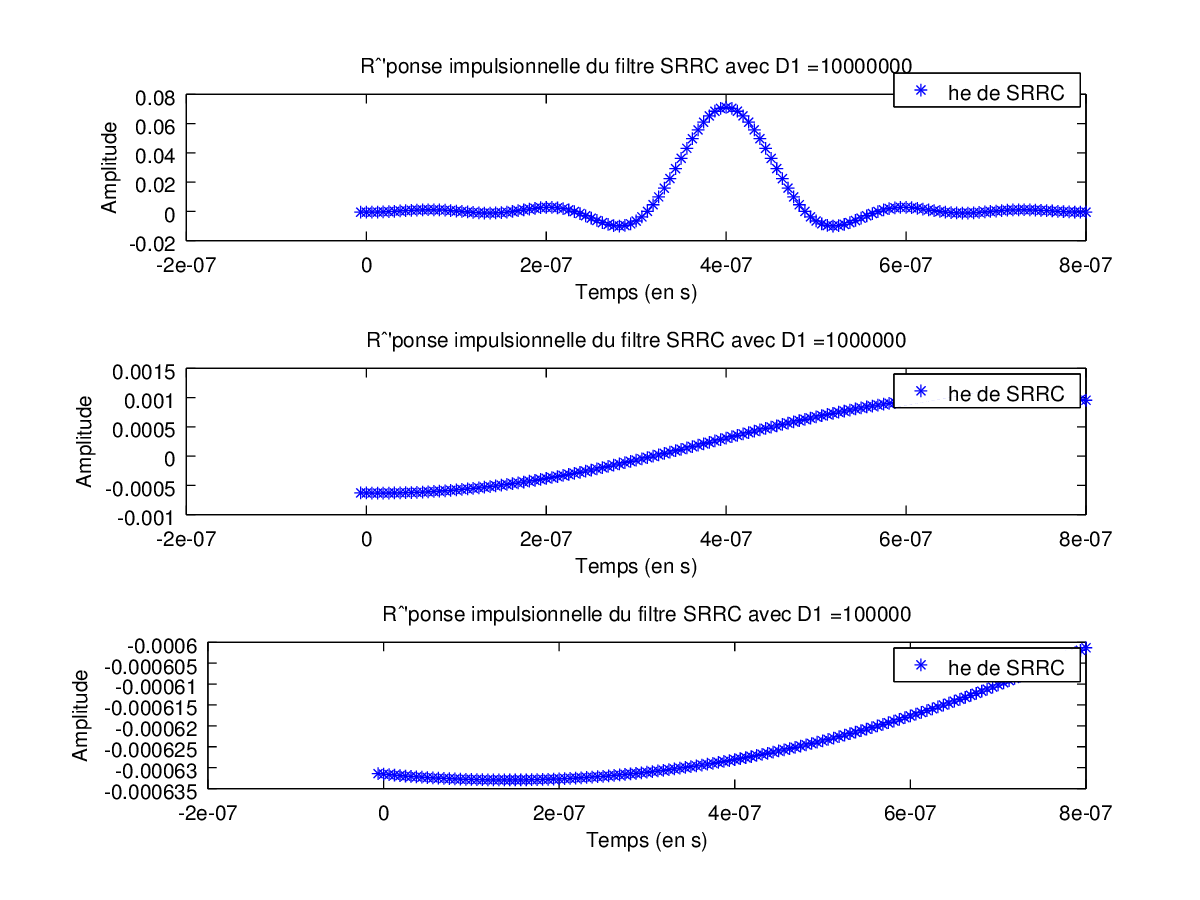
\includegraphics[scale=0.45]{SRRC_varD_3.png}
\end{center}

Interêt de D : 

\begin{center}
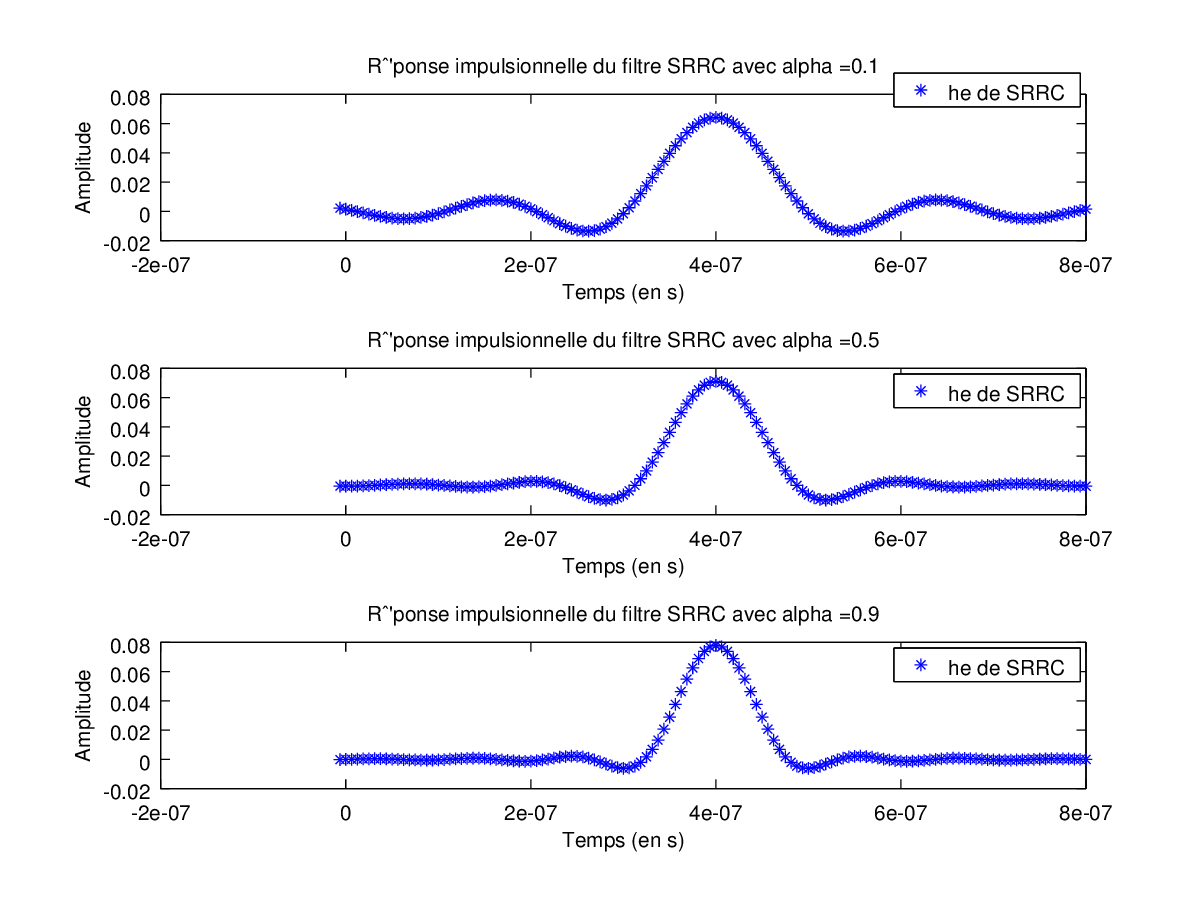
\includegraphics[scale=0.45]{SRRC_varAlpha_3.png}
\end{center}

Interêt de alpha :

Est-ce logique d'observer une variation de phase linéaire avec la fréquence ?

\subsection{Mise en forme des symboles}

\subsubsection{Question 3}
\begin{lstlisting}
t_x = -L*F*T/2 : T : (N*F)*T + L*F*T/2;
ht = gen_filters2('srrc',t_filtre,T,F,L,0.5);
xt = conv(st, ht);
figure; subplot(2,1,1); plot(t_s, st, '*'); subplot(2,1,2); plot(t_x, xt);
\end{lstlisting}

\begin{center}
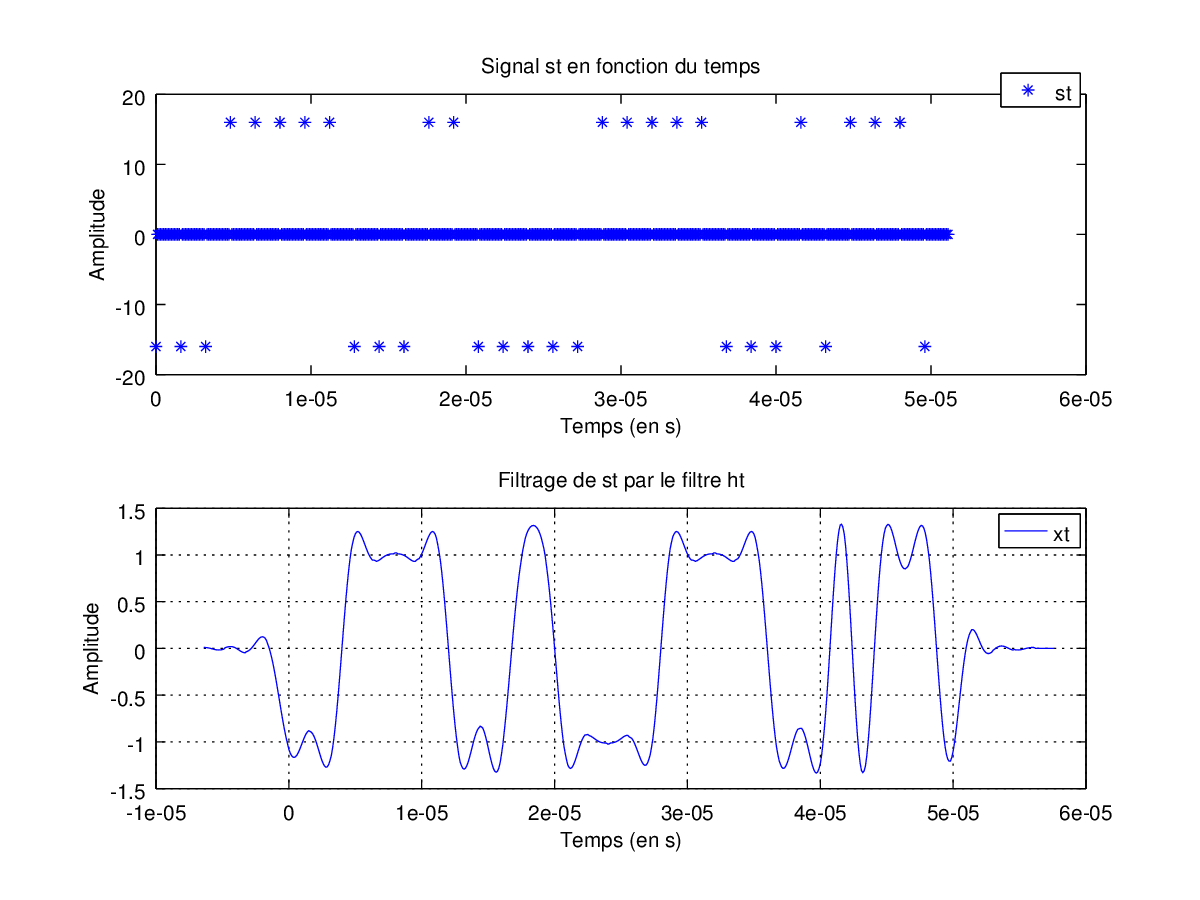
\includegraphics[scale=0.45]{conv_3_3.png}
\end{center}

\begin{lstlisting}
length(st)
length(ht)
length(t_x)*T
length(t_filtre)*T
\end{lstlisting}

Résultats : ans =  512
ans =  130
ans =    6.4100e-05
ans =    1.3000e-05

\subsubsection{Question 4}
\begin{lstlisting}
mean(xt.^2)
\end{lstlisting}

Résultat : 1 -> cohérent avec la théorie car la variance vaut 1 et le norme carrée du filtre d'émission vaut 1/T (filtre normalisé)

\subsubsection{Question 5}

\subsubsection{Question 6}


\section{Ajout du bruit blanc gaussien - Question 7}

On sait que sigman² = (No*F)/(2*T)
or P(xt) = Eb/T d'où la formule

De plus, on a P(xt) = 1 ici donc sigman² = f(Eb/N0) avec f(x) = F/(2*x)

\begin{lstlisting}
sigma_n = sqrt((F/2)/(10.^(EbNodB/10)));
nt=sigma_n*randn(1,length(xt));
rt = xt + nt;
\end{lstlisting}

\begin{center}
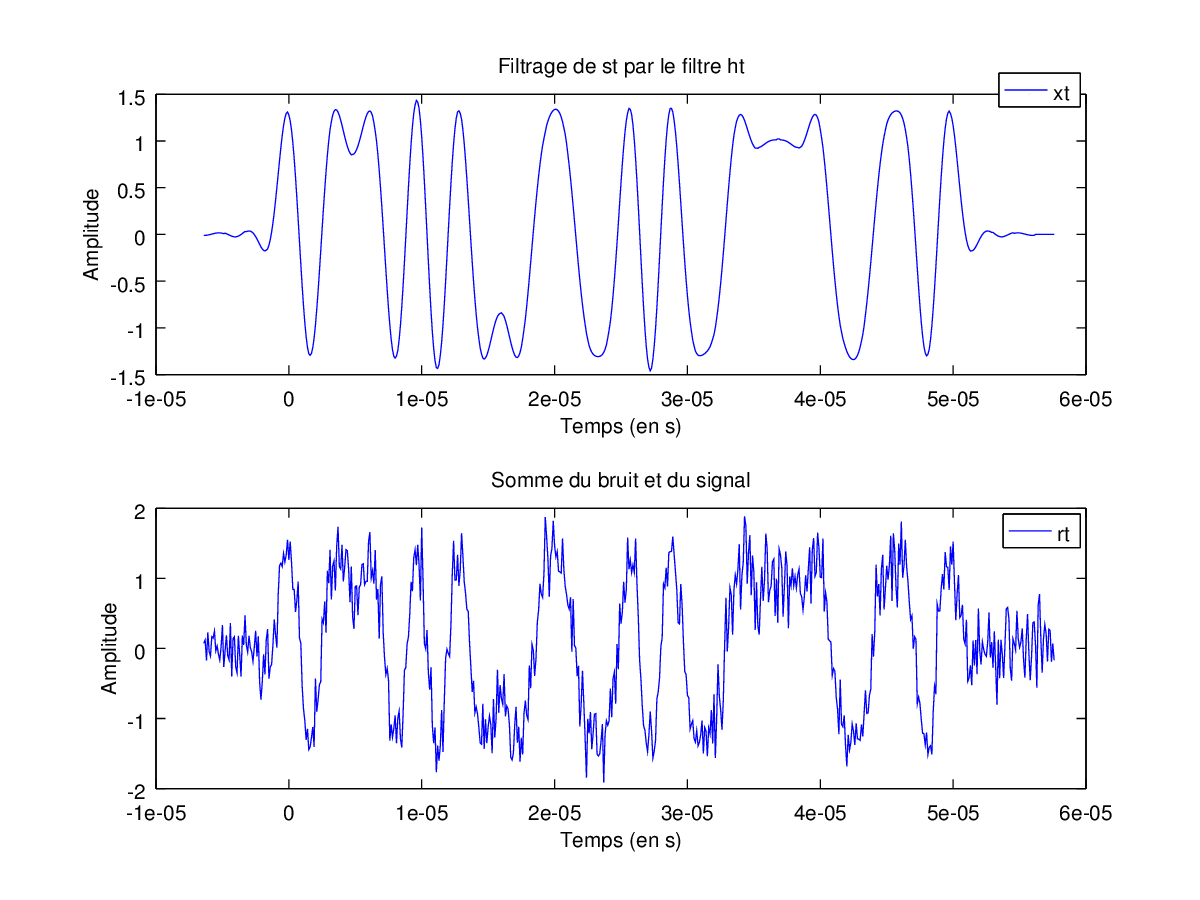
\includegraphics[scale=0.45]{signalBruite_7.png}
\end{center}


\section{Conversion analogique - numérique}
\subsection{Filtrage adapté}
\subsection{Décimation}


\section{Prise de décision (demapping)}


\section{Calcul du taux d'erreur binaire}


\section{Mesures de performances}


\section{Optionnel}
\subsection{Autres impulsions de mise en forme}
\subsection{Rapport signal à bruit sur la variable de décision}
\subsection{Analyseur de spectre}


\section{Conclusion}

\bibliographystyle{abbrv}
\bibliography{sigproc}  % sigproc.bib is the name of the Bibliography in this case
\nocite{*}

\balancecolumns
% That's all folks!
\end{document}
